\section{Design}

This section outlines the overall design of our project, including the architecture, technology stack, and deployment process. We also discuss the cloud provider, infrastructure, version control, and continuous integration/continuous delivery (CI/CD) practices employed. 

\subsection{Overview}

Our system comprises three main layers: the front-end UI layer, the API layer, and the back-end layer. The front-end UI layer is the user-facing component of our application and is hosted as a web application. It provides a graphical user interface that enables users to interact with the system and access the necessary information. 

As seen in \autoref{fig:sequence-diagram}, the API layer is hosted on Azure and is implemented using .NET. It serves as the communication interface between the front-end UI and back-end layers. The API layer receives requests from the front-end UI layer, processes them, and sends them to the back-end layer for data retrieval and processing. The API layer also handles authentication and authorization, ensuring that users only have access to the data they are authorized to view. 

The back-end layer is hosted on AWS and is responsible for storing and processing data. It comprises various services and components, including databases, storage systems, and compute resources. The back-end layer receives requests from the API layer, processes them, and sends the results back to the API layer for transmission to the front-end UI layer. 

We can achieve better scalability, maintainability, and fault tolerance by splitting our system into these three layers. The separation of concerns also makes adding new features and functionality to the system easier over time. 

\begin{figure}[htp]
    \centering
    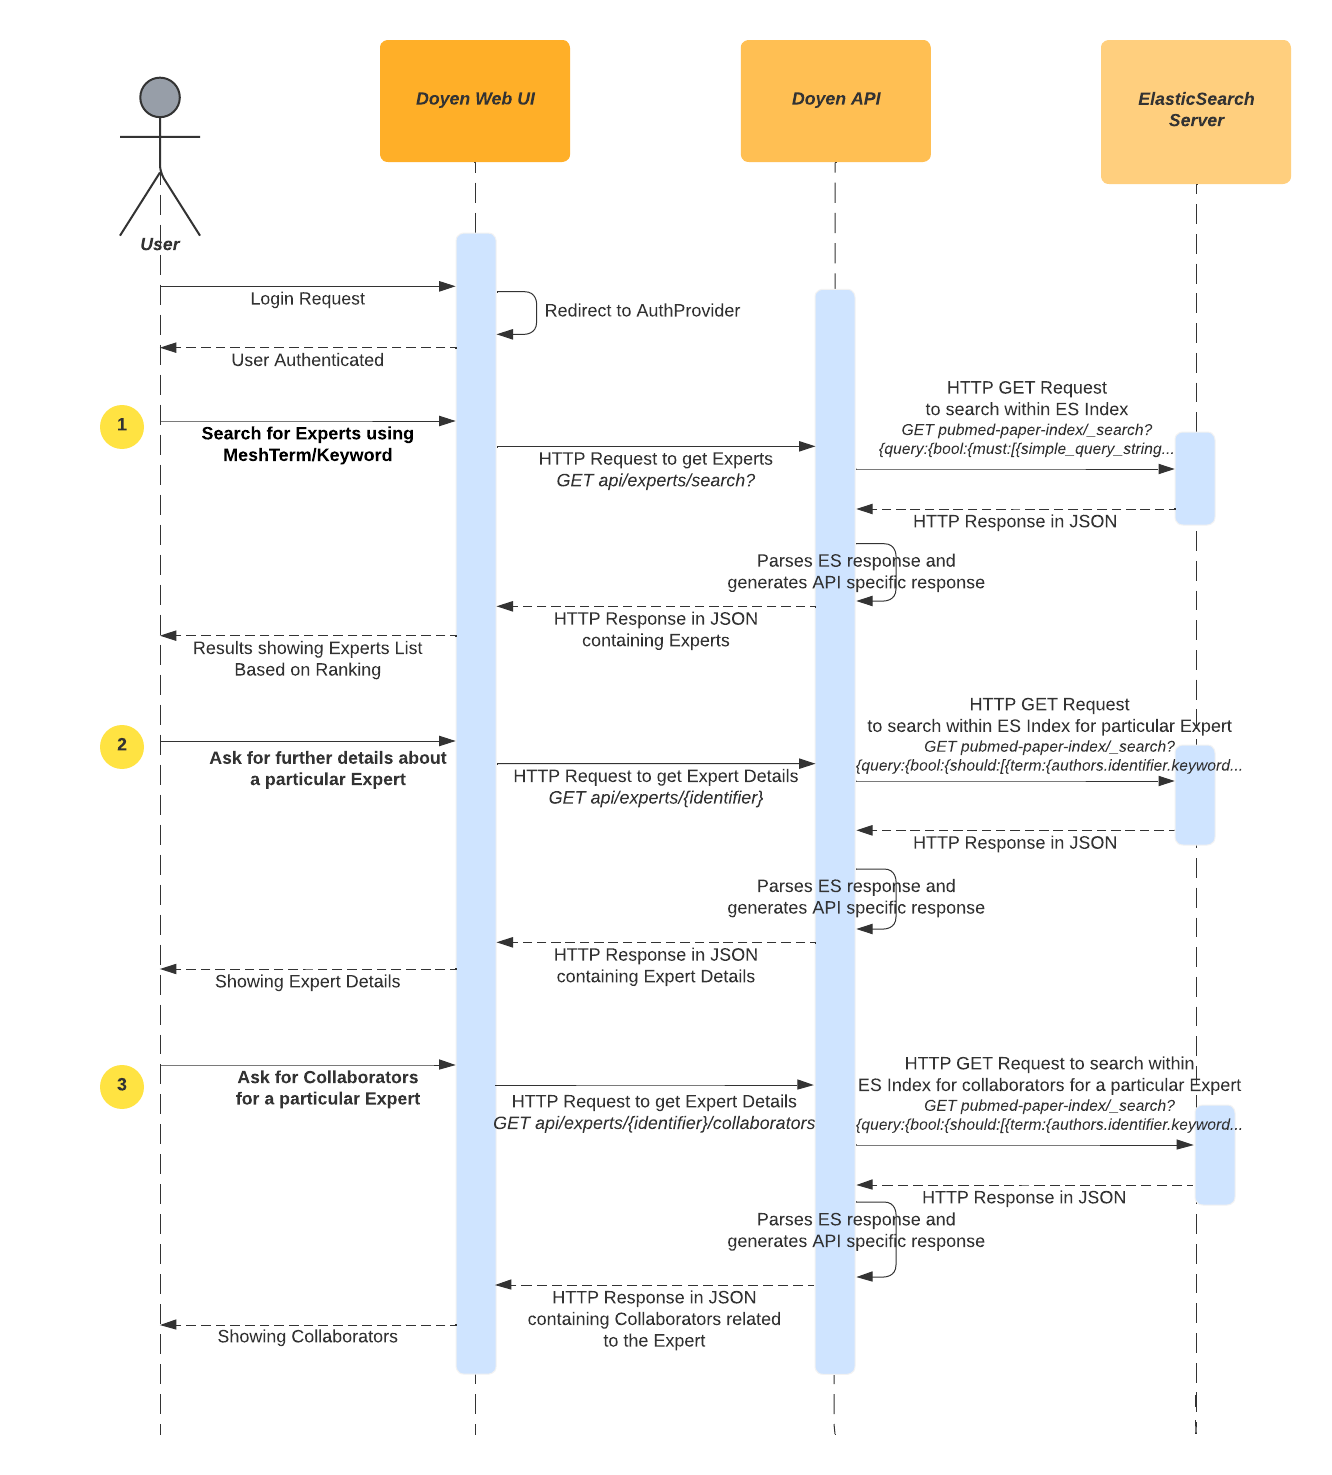
\includegraphics[width=\textwidth]{Images/SequenceDiagram_GetExperts.png}
    \caption[A Sequence Diagram of the End-to-end Flow]{\textbf{A Sequence Diagram of the End-to-end Flow:} The sequence diagram represents the sequence of steps involved in the user's login and search interactions with the system. It demonstrates the flow of requests and responses between the various components, showcasing the communication between the User and the different layers represented by respective components. }
    \label{fig:sequence-diagram}
\end{figure}


\subsection{Front-End}

For the front-end of our application, we chose to implement the client using Next.js 13, a popular and efficient React framework for building user interfaces. Next.js allows us to create modular and reusable components, enhancing our application's development speed and maintainability. 

In addition to Next.js, we utilized Tailwind CSS as our front-end styling framework. Tailwind is a highly customizable, low-level CSS framework that promotes a utility-first approach to styling. This choice enabled us to quickly build consistent, responsive, and performant user interfaces with minimal CSS overhead. 

\subsection{Back-End}

Our back-end services are hosted on Amazon Web Services (AWS) EC2 instance and Azure. AWS EC2 allows users to launch Virtual Machines on the Amazon Cloud infrastructure with various workloads and application combinations. This choice allows us to focus on our application's functionality while AWS handles the scaling and maintenance of the underlying infrastructure. The API Gateway is the entry point for our back-end services, providing a fully managed service for creating, publishing, and maintaining secure APIs. 

We implemented our data ingestion layer using PySpark, a Python library for Apache Spark. PySpark allows us to process large-scale data in parallel, enabling efficient data manipulation and transformation. Furthermore, we built our ingestion pipeline using Python. 

The back-end service API layer is implemented in .Net using C\# and hosted on Microsoft Azure Cloud. This combination enables us to build scalable and maintainable server-side applications while leveraging the vast Microsoft .Net libraries and tools ecosystem. 

\subsection{Ingestion Pipeline}

Our system has an ingestion pipeline workflow, shown in \autoref{fig:ingestion-flow}, which automatically downloads baseline data from the PubMed FTP server and processes it. The processed data is then stored in an Elasticsearch instance hosted on an EC2 instance inside a Docker container. The ingestion pipeline is also located on the same EC2 instance and runs on demand. 

To keep the Elasticsearch index up-to-date, we have implemented a daily cron job that downloads the daily update PubMed file from the Ftp server and runs the same ingestion pipeline. This ensures that the Elasticsearch index is always up-to-date and reflects the latest changes in the PubMed database. 

By automating the data ingestion process and implementing the daily cron job, we have reduced the manual effort required to update the Elasticsearch index, minimized the risk of errors and inconsistencies, and ensured that our system is constantly working with the most up-to-date data. 

\begin{figure}[htp]
    \centering
    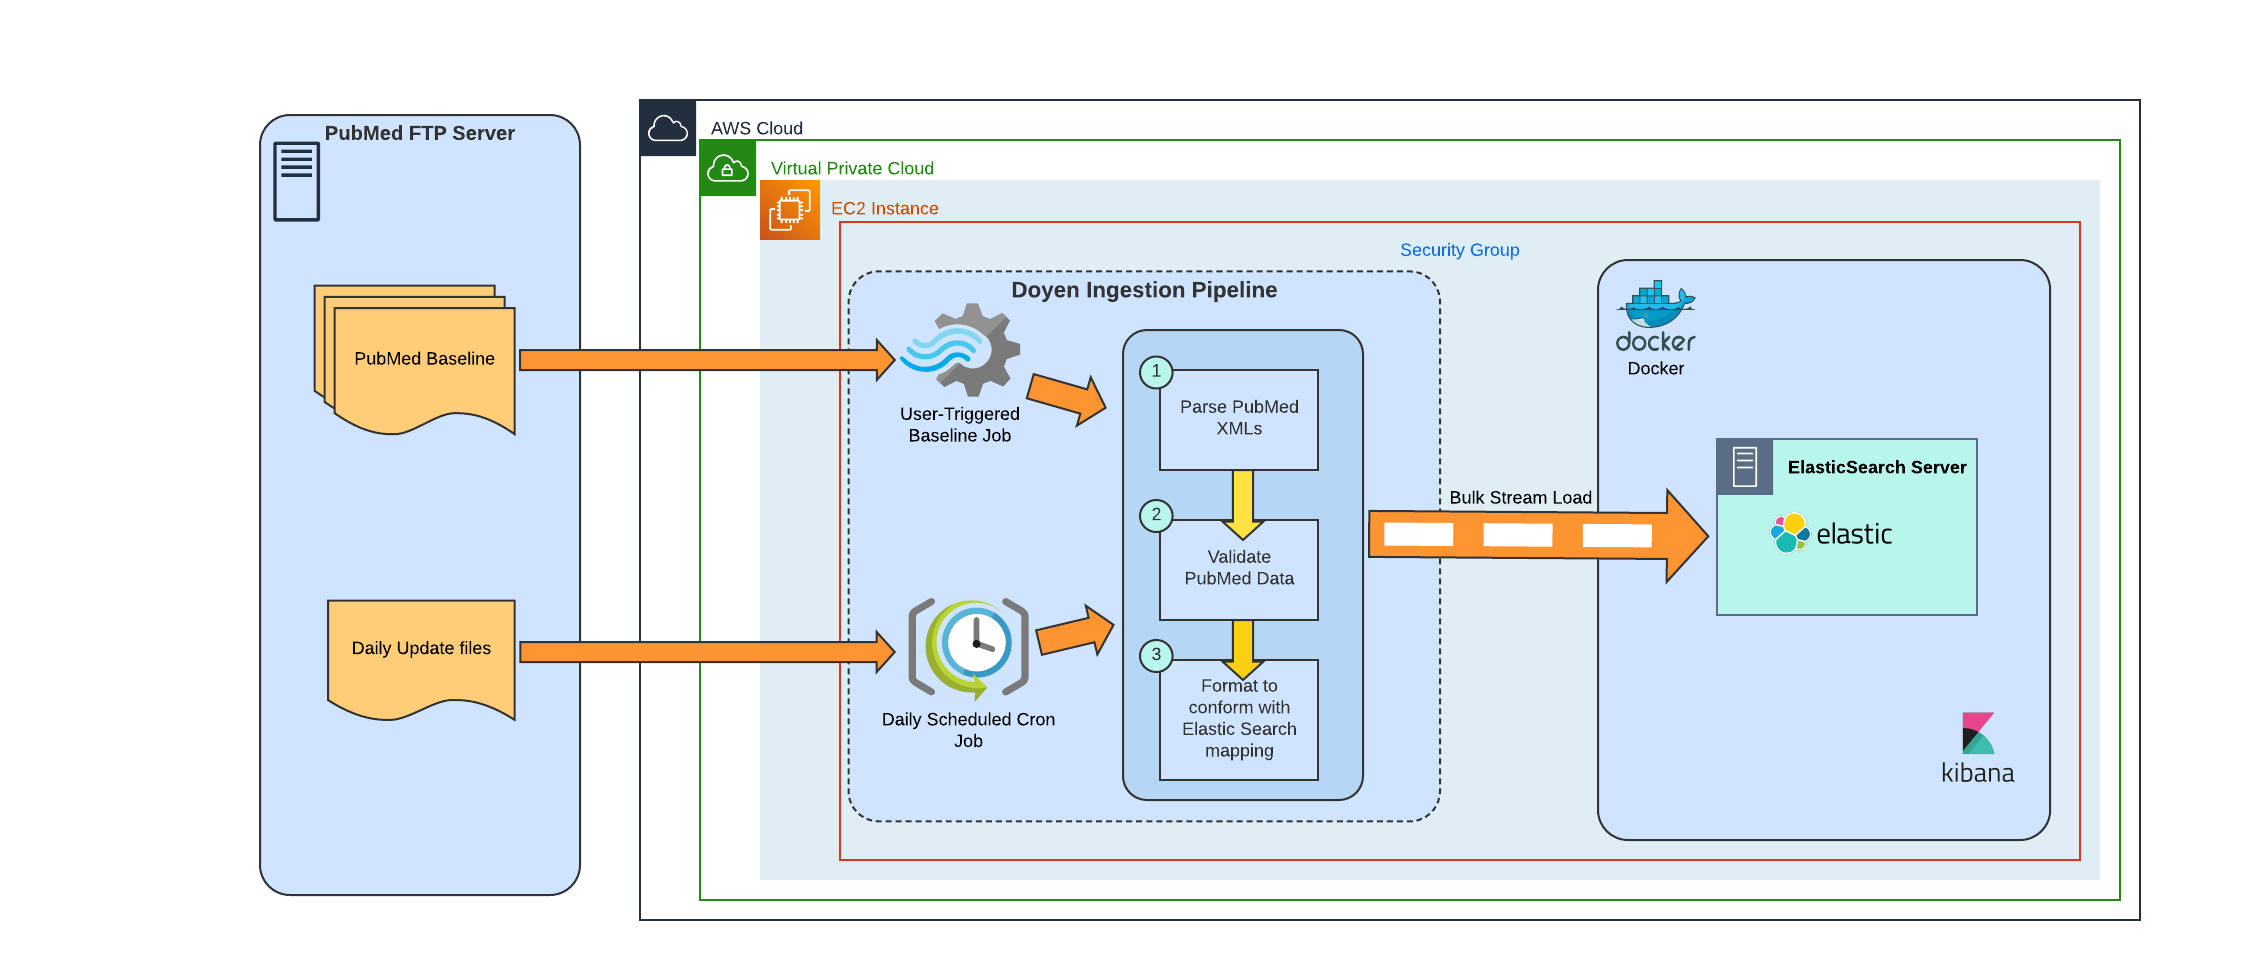
\includegraphics[width=\textwidth]{Images/Ingestion Pipeline flow.png}
    \caption[A Diagram of the Ingestion Pipeline Flow]{\textbf{A Diagram of the Ingestion Pipeline Flow:} The flow diagram displayed in the above figure represents the Ingestion pipeline workflow of our system. The pipeline is responsible for automatically downloading baseline data from the PubMed FTP server, processing it, and storing the processed data in an Elasticsearch instance. The process begins with the ingestion pipeline fetching the baseline data from the PubMed FTP server. The downloaded data is then passed through various processing steps to transform and prepare it for storage. Once the data has been processed, it is stored in an Elasticsearch instance that is hosted on an EC2 instance and is encapsulated within a Docker container. This setup provides a scalable and isolated environment for efficiently storing and querying the processed data. To ensure that the Elasticsearch index remains up-to-date with the latest changes in the PubMed database, a daily cron job has been set up to download the daily update PubMed file from the FTP server and triggers the same ingestion pipeline. }
    \label{fig:ingestion-flow}
\end{figure}


In \autoref{fig:ingestion}, the Ingestion Pipeline comprises several classes, with the main entry point being the PubmedProcessor class. This class contains functions to create the Elasticsearch PubMed index and ingest files, utilizing the Elasticsearch and NihFtpClient libraries. 

\begin{figure}[htp]
    \centering
    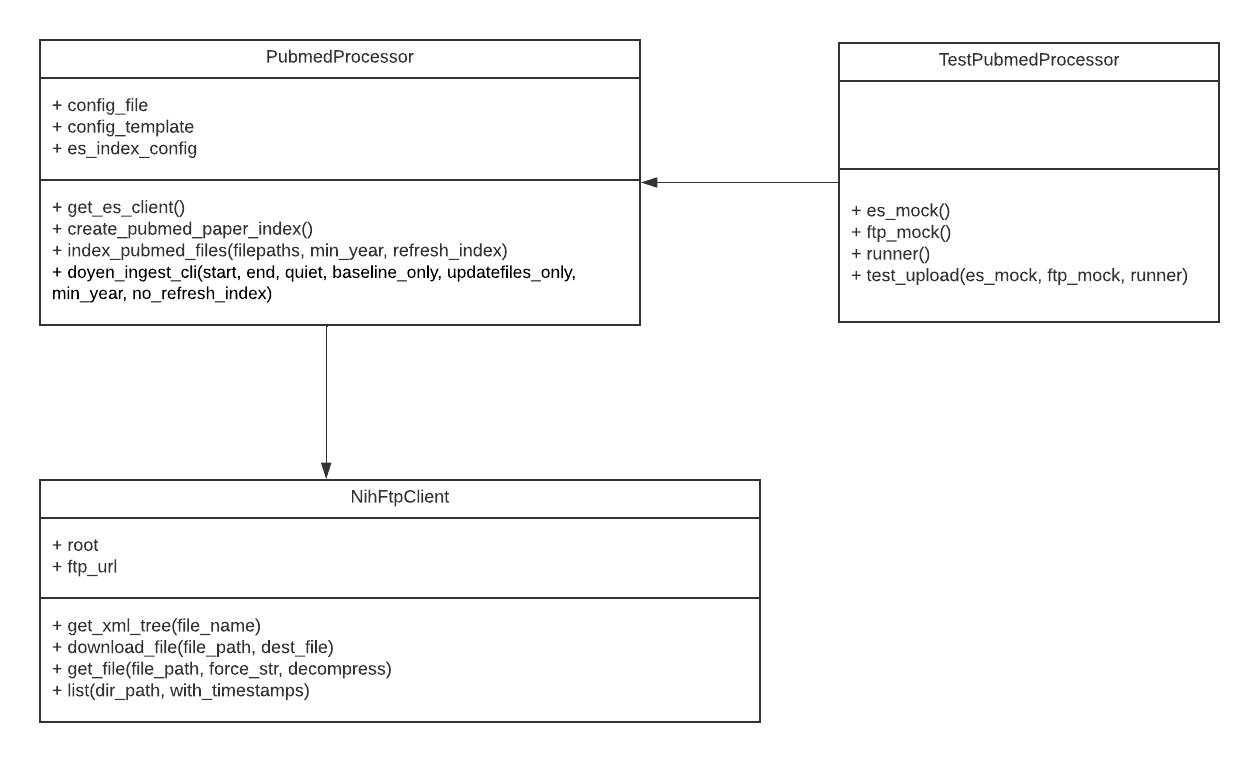
\includegraphics[width=\textwidth]{Images/IngestionPipeline_ClassDiagram.png}    
    \caption[A Class Diagram of the Ingestion Pipeline Model]{\textbf{A Class Diagram of the Ingestion Pipeline Model:} The class diagram displayed in the above figure represents the Ingestion Pipeline model for processing PubMed data. It consists of three classes: \emph{PubmedProcessor}, \emph{NihFtpClient}, and \emph{TestPubmedProcessor}. \emph{PubmedProcessor} is responsible for retrieving FTP data from PubMed FTP by utilizing the \emph{NihFtpClient} class. It further processes the data and performs the ingestion into Elasticsearch. The \emph{PubmedProcessor} class acts as the main component of the pipeline, coordinating the data retrieval, processing, and ingestion tasks. The \emph{NihFtpClient} class serves as a utility class, providing the necessary functionality to communicate with the PubMed FTP server and retrieve the required data. It acts as a bridge between \emph{PubmedProcessor} and the PubMed FTP server. Additionally, there is a \emph{TestPubmedProcessor} class included in the diagram, which contains unit tests for the \emph{PubmedProcessor} class.}
    \label{fig:ingestion}
\end{figure}



\subsection{API Layer}

The API layer, shown in \autoref{fig:api-layer}, is a crucial component facilitating communication between the front-end and back-end. It serves as the primary interface for the front-end to interact with the back-end services. The API layer manages and processes incoming requests from the front-end and sends them to the Elasticsearch Server for data retrieval. It executes queries against the server to retrieve the desired data and refines and translates it into a format easily digestible for the front-end. 

Apart from basic search queries, the API layer is also responsible for running advanced queries, such as aggregated queries, extracting expert-related information like collaborators, research interests, and more. The API layer provides a seamless user experience, ensuring data is processed and delivered efficiently and accurately. It also allows the system to be extensible, bringing in additional or changing data sources to supplement current data without breaking the interface to the UI. 


\begin{figure}[htp]
    \centering
    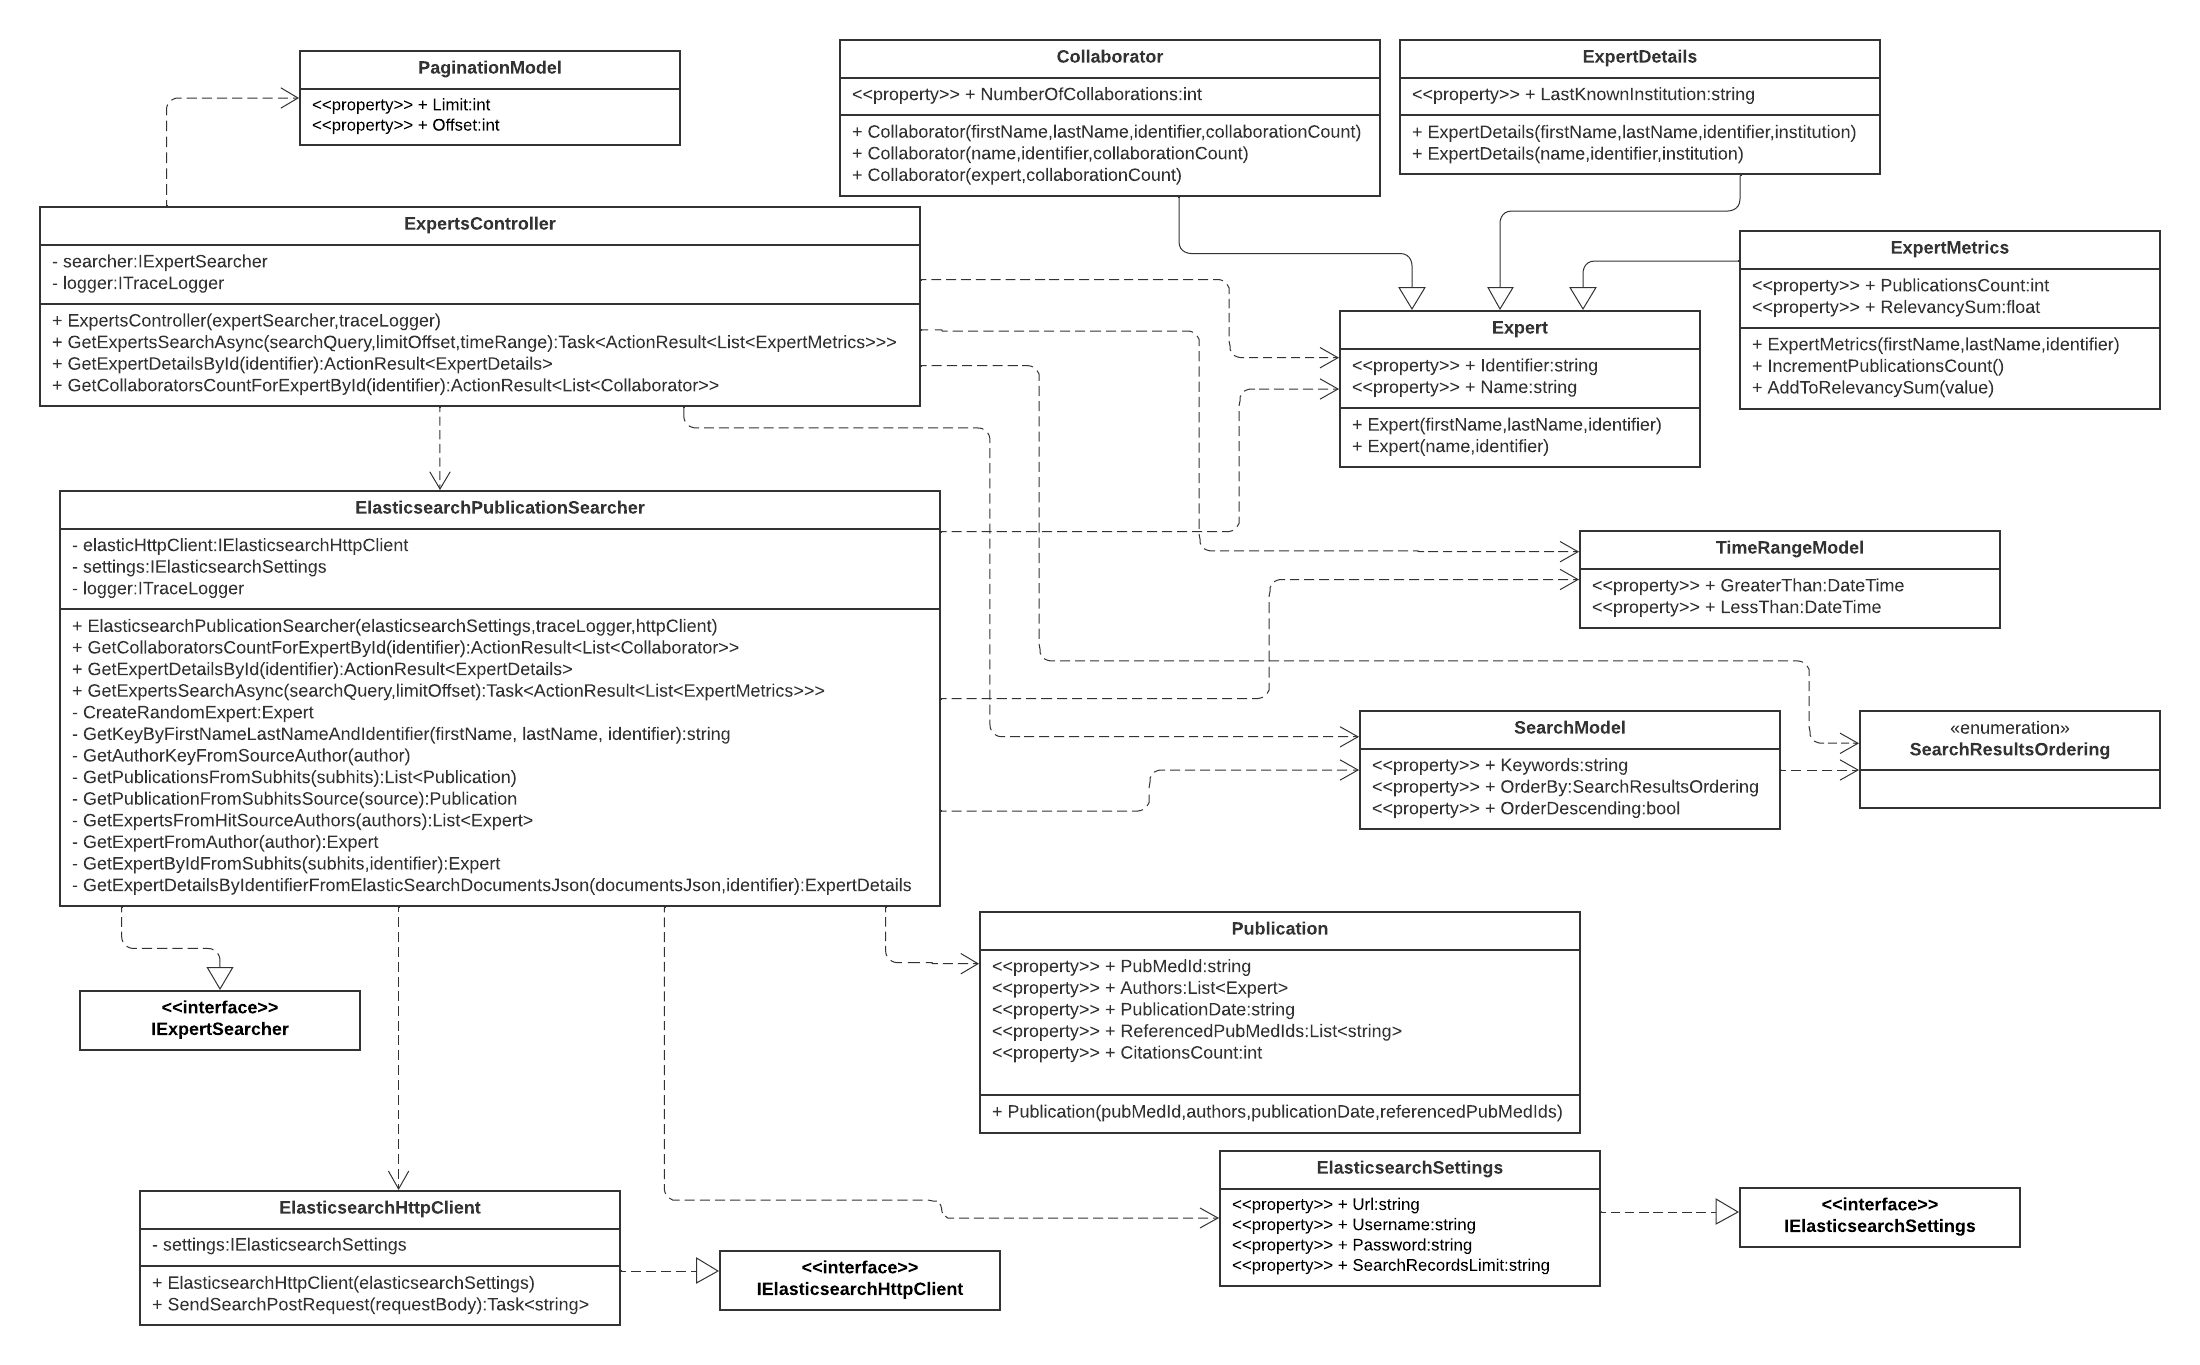
\includegraphics[width=\textwidth]{Images/API_ClassDiagram.png}    
    \caption[A Class Diagram of the API Layer]{\textbf{A Class Diagram of the API Layer:} Illustration of the classes and their relationships in the API layer serving as an interface between the back-end and front-end. The class diagram displayed above represents the API layer, which acts as an interface between the back-end and front-end components of the system. The diagram includes several classes involved in this layer, namely \emph{ExpertsController}, \emph{ElasticsearchPublicationSearcher}, and \emph{ElasticsearchHttpClient}. The \emph{ExpertsController} class serves as the API controller and contains methods responsible for handling requests related to experts. It provides functionality to retrieve a list of experts based on a provided query and to obtain details and collaborators for a specific expert. The \emph{ElasticsearchPublicationSearcher} class is responsible for retrieving expert-related data from Elasticsearch. It is utilized by the \emph{ExpertsController} class to obtain the necessary information. The \emph{ElasticsearchPublicationSearcher} class interacts with Elasticsearch using the \emph{ElasticsearchHttpClient} class. The \emph{ElasticsearchHttpClient} class acts as a utility class for making HTTP queries against the Elasticsearch server. It enables the \emph{ElasticsearchPublicationSearcher} class to send requests and receive responses from the Elasticsearch server, allowing the retrieval of the required expert data. }
    \label{fig:api-layer}
\end{figure}

\subsection{Data Management}

Our primary data is hosted and searched using Elasticsearch, a powerful and flexible search and analytics engine. Elasticsearch allows us to store, search, and analyze large volumes of data quickly and in near real-time.

\subsection{Cloud Provider}

For our cloud provider, we selected Amazon Web Services (AWS). AWS offers a comprehensive suite of tools and services to help us build, deploy, and manage our applications effectively and securely. 

\subsection{Infrastructure}

As previously mentioned, our primary data is hosted in Elasticsearch. To manage our resource deployments, we utilized AWS CloudFormation, enabling us to create and manage a collection of AWS resources using templates. This approach helped streamline infrastructure management and ensure a consistent and reproducible environment. The overall architecture is shown in \autoref{fig:architecture}.

Our back-end is hosted on AWS Lambda and served through Amazon API Gateway, as discussed in section 2.2. We also use AWS CloudFront, a global content delivery network (CDN) service, to serve our front-end. CloudFront accelerates the delivery of our application's assets by caching and distributing them across a network of edge locations, improving the overall user experience. 

\begin{figure}[htp]
    \centering
    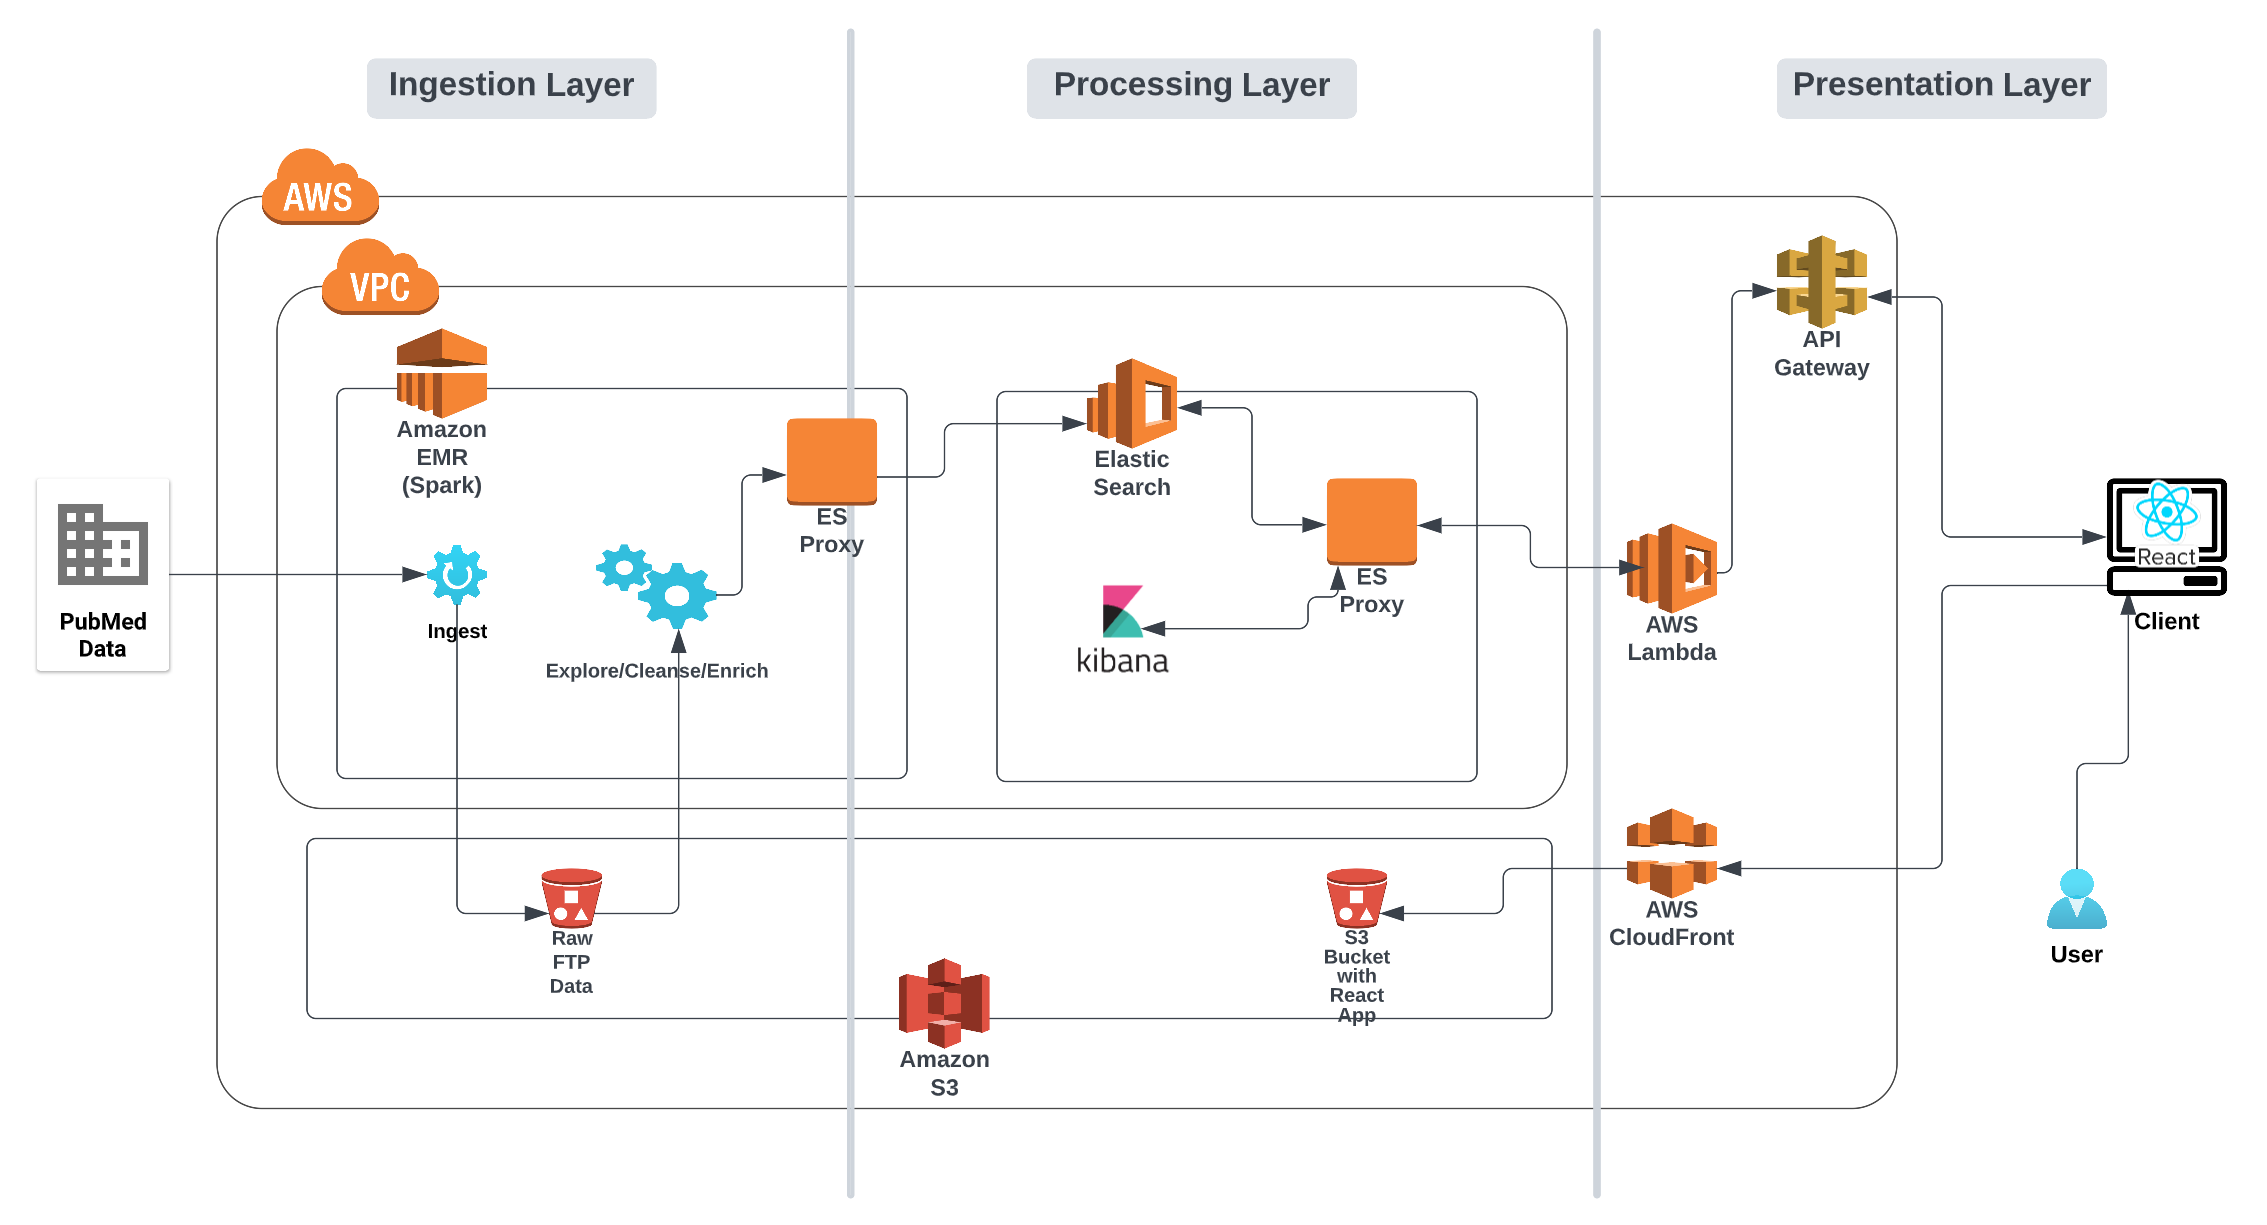
\includegraphics[width=\textwidth]{Images/Doyen High-Level Architecture Diagram.png}
    \caption{The Doyen Architecture}
    \label{fig:architecture}
\end{figure}

\subsection{Version Control and CI/CD}

We used GitHub for version control, allowing us to manage our codebase effectively, track changes, and collaborate efficiently. GitHub also implements our continuous integration/continuous delivery (CI/CD) pipeline. This pipeline automates the process of building, testing, and deploying our application, ensuring we maintain a high code quality and consistency throughout the project's lifecycle. By implementing a CI/CD pipeline, we can detect and address issues early, reduce manual intervention, and streamline the delivery of new features and bug fixes. 

In conclusion, our project's design incorporates modern and scalable technologies to ensure a robust and maintainable application. Our choice of AWS as a cloud provider, combined with implementing CloudFormation, CloudFront, and a CI/CD pipeline using GitHub, allows us to streamline our infrastructure management and ensure a consistent and reproducible environment for our application. By utilizing Next.js, Tailwind CSS, Elasticsearch, AWS Lambda, and API Gateway, we built an efficient and responsive front-end and a reliable and scalable back-end to manage our data effectively. 